\section{Comparison Dimension Reduction} \label{sec:Comparison_Dimension_Reduction}

\blindtext

\begin{figure}[!hbt]
    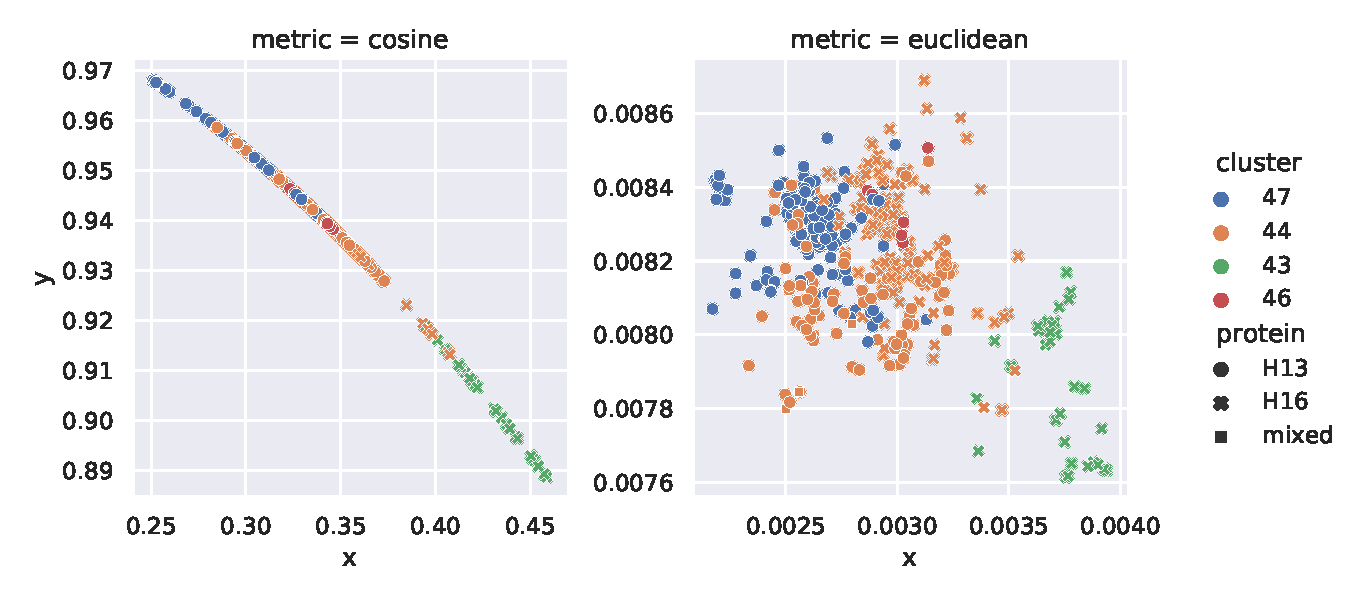
\includegraphics[width=\dimexpr\textwidth-2\fboxsep-2\fboxrule,fbox]{PCA/Difference_Segment_4_H_PCA.pdf}
    \caption[H13/H16 Component Reduction Example with \Acrshort{PCA}]{\textbf{H13/H16 Component Reduction Example with \Acrshort{PCA}.} .}
    \label{fig:Reduction_Example_PCA}
\end{figure}

\begin{figure}[!hbt]
    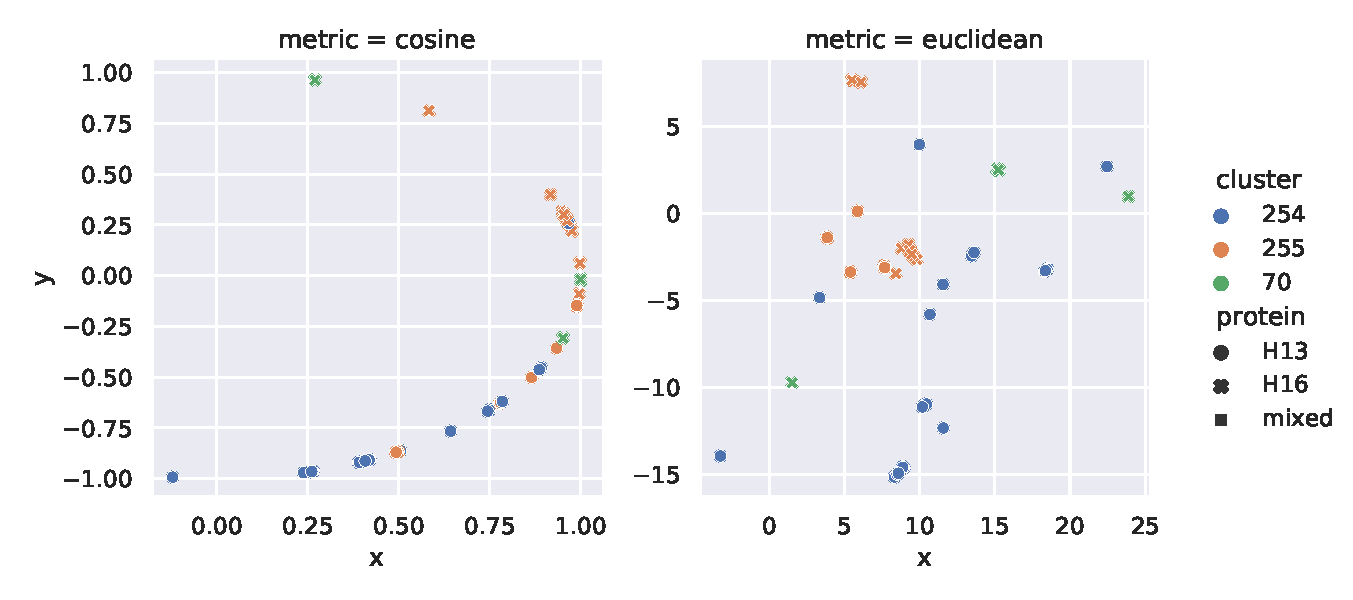
\includegraphics[width=\dimexpr\textwidth-2\fboxsep-2\fboxrule,fbox]{UMAP/Difference_Segment_4_H_UMAP_Neighbors_10.pdf}
    \caption[H13/H16 Component Reduction Example with \Acrshort{UMAP} (n = 10)]{\textbf{H13/H16 Component Reduction Example with \Acrshort{UMAP} (n = 10).} .}
    \label{fig:Reduction_Example_UMAP_10}
\end{figure}

\begin{figure}[!hbt]
    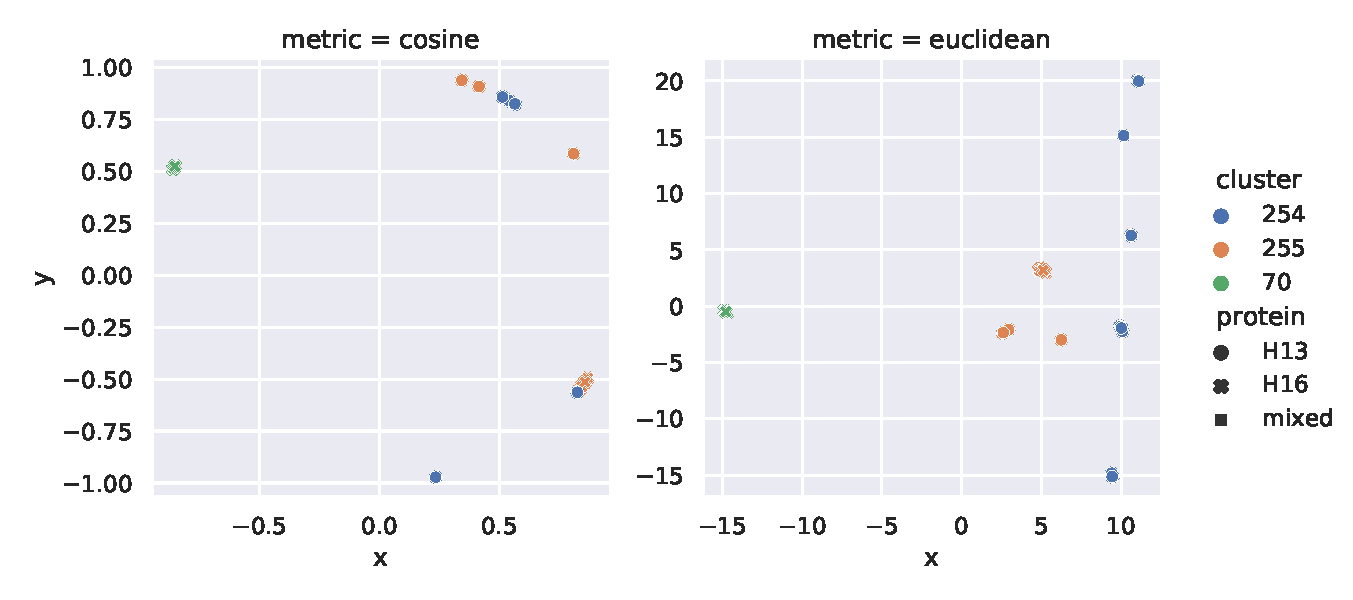
\includegraphics[width=\dimexpr\textwidth-2\fboxsep-2\fboxrule,fbox]{UMAP/Difference_Segment_4_H_UMAP_Neighbors_50.pdf}
    \caption[H13/H16 Component Reduction Example with \Acrshort{UMAP} (n = 50)]{\textbf{H13/H16 Component Reduction Example with \Acrshort{UMAP} (n = 50).} .}
    \label{fig:Reduction_Example_UMAP_50}
\end{figure}

\begin{figure}[!hbt]
    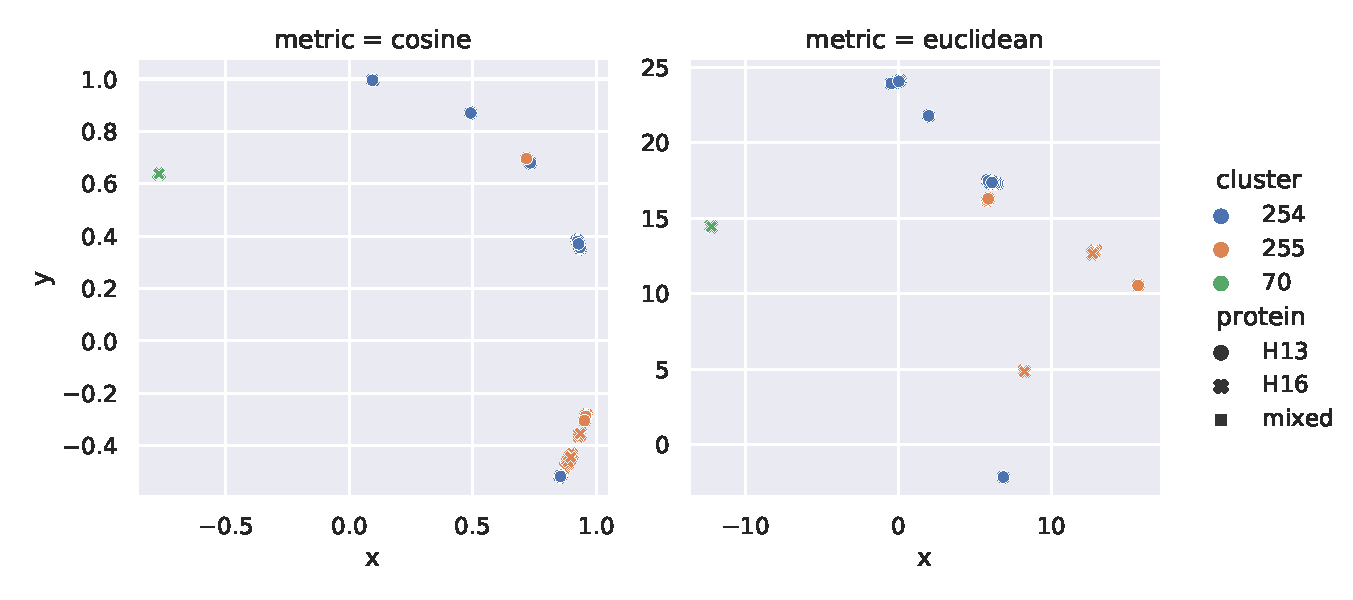
\includegraphics[width=\dimexpr\textwidth-2\fboxsep-2\fboxrule,fbox]{UMAP/Difference_Segment_4_H_UMAP_Neighbors_100.pdf}
    \caption[H13/H16 Component Reduction Example with \Acrshort{UMAP} (n = 100)]{\textbf{H13/H16 Component Reduction Example with \Acrshort{UMAP} (n = 100).} .}
    \label{fig:Reduction_Example_UMAP_100}
\end{figure}

\begin{figure}[!hbt]
    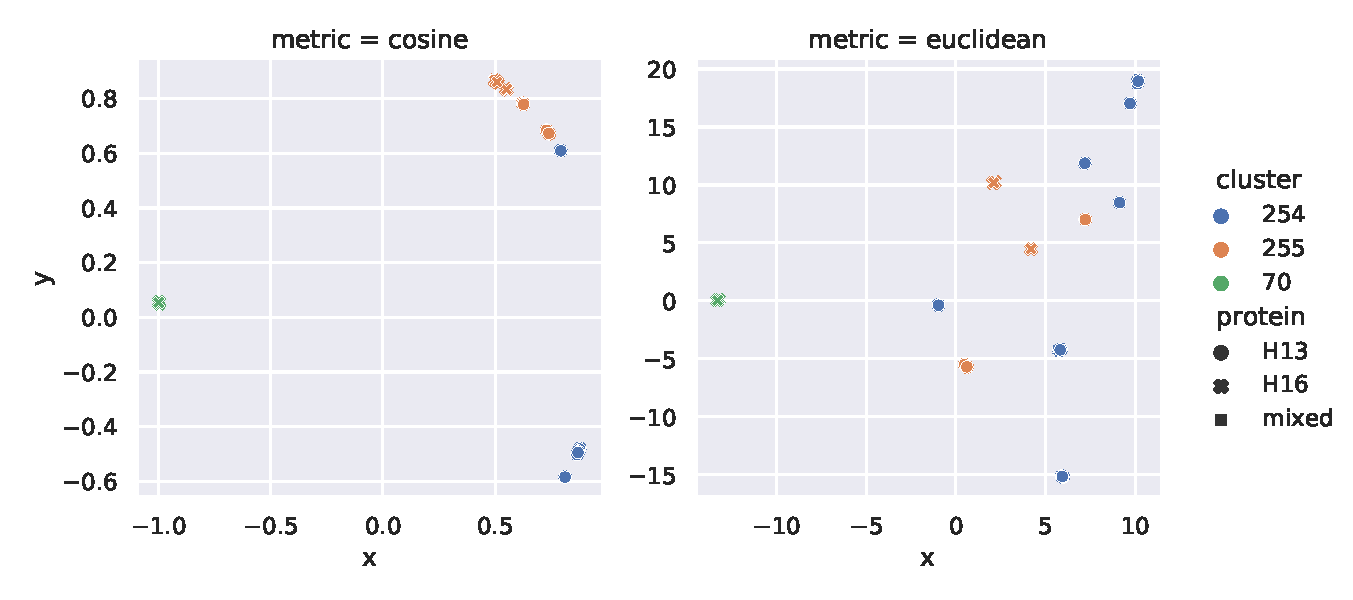
\includegraphics[width=\dimexpr\textwidth-2\fboxsep-2\fboxrule,fbox]{UMAP/Difference_Segment_4_H_UMAP_Neighbors_200.pdf}
    \caption[H13/H16 Component Reduction Example with \Acrshort{UMAP} (n = 200)]{\textbf{H13/H16 Component Reduction Example with \Acrshort{UMAP} (n = 200).} .}    \label{fig:Reduction_Example_UMAP_200}
\end{figure}